\chapter{Postulats \& applications}

\paragraph{Exercice 1} \textit{Évolution quantique.}\\
Soit un système quantique dont l'état dépendant du temps est noté $\ket{\psi(t)}$, et dont l'opérateur Hamiltonien s'écrit $\hat H(t)$. 
\begin{enumerate}
\item \textbf{Opérateur d'évolution.}
\begin{enumerate}
\item Déduisez de l'uniformité du temps de la Relativité Galiléenne qu'il existe un opérateur unitaire $\hat U(t,t_0)$ qui fasse évoluer l'état $\ket{\psi(t)}$ du temps $t_0$ de référence au temps $t\geq t_0$. 
\item Prouvez que cet $\hat U(t,t_0)$ est unique, et ne dépend donc pas de l'état de départ $\ket{\psi(t_0)}$.
\item Montrez que l'ensemble de tels opérateurs $\hat U(t,t_0)$ doit former un groupe à un paramètre pour la loi de composition des opérateurs agissant sur l'espace des états du système.
\end{enumerate} 
\item \textbf{Évolution des états quantiques.}
\begin{enumerate}
\item Montrez que l'équation d'évolution d'un état quantique $\ket{\psi(t)}$ est de la forme 
\begin{equation}
i\hbar \frac{\partial}{\partial t}\ket{\psi(t)} = \hat A(t,t_0)\ket{\psi(t)}
\end{equation}
pour un opérateur $\hat A(t,t_0)$ que l'on calculera en fonction de $\hat U(t,t_0)$.
\item Démontrez que $\hat A(t,t_0)$ est hermitien et indépendant de $t_0$. On notera donc $\hat A(t)$.
\item Justifiez, grâce au Principe de Correspondance \textit{et} la définition de $\hat H$ que $\hat A(t) = \hat H(t)$ est un choix physiquement raisonnable. Qu'avez-vous retrouvé ?
\item Donnez l'expression de $\hat U(t,t_0)$ pour un système conservatif (le cas général fait l'objet d'un calcul assez technique qui ne sera pas abordé ici). 
\item Pouvez-vous interpréter le rôle de l'opérateur $\hat H$ ?
\end{enumerate}
\end{enumerate}


\paragraph{Exercice 2} \textit{Théorème d'Ehrenfest.}
\begin{enumerate}
\item Soit l'observable $\hat O$ agissant dans l'espace des états du système. Dérivez l'équation d'évolution de la valeur moyenne de $\hat O$ dans l'état $\ket{\psi(t)}$.
\item Explicitez cette équation pour $\hat O = \hat{\vec{P}}$ et $\hat O = \hat{\vec{X}}$, et montrez que cela conduit aux équations de Hamilton pour les valeurs moyennes de ces observables. 
\item Considérez une particule libre à une dimension possédant, à l'instant initial $t=0$, une quantité de mouvement $p_0$.
\begin{enumerate}
\item Montrez que les valeurs moyennes de $\hat P(t)$ et $\hat X(t)$ évoluent conformément aux équations classiques.
\item Montrez que $m \frac{d}{dt}\braket{\hat X^2} = 2\braket{\hat P\hat X} + i\hbar$. Comment $\braket{\hat P^2}$ évolue-t-elle ?
\item Déduisez-en que l'étalement $\Delta x$ du paquet d'onde décrivant la particule est une fonction quadratique en $t$. Cela vous rappelle-t-il quelque chose ?
\end{enumerate}
\end{enumerate}
$ $
%\item Dans la \textbf{Représentation de Heisenberg}, ce ne sont pas les états mais bien les observables qui portent toute la dépendance temporelle. Déterminez dans ce cas l'équation d'évolution d'une observable $\hat Q(t)$ agissant sur le système dans cette représentation (\textit{équation de Heisenberg}). Particularisez à $\hat Q =  \hat{\vec X}$ et $\hat Q = \hat{\vec P}$. Commentaires ?



\paragraph{Exercice 3} \textit{Opérateurs position et quantité de mouvement.} \\
En mécanique classique, le mouvement d'une particule se déplaçant dans l'espace est formulé en termes d'un espace des phases dont les coordonnées sont $(\vec x,\vec p)$, où $\vec p$ est le moment canoniquement conjugué à $\vec x$, appelé quantité de mouvement. \\

Par le truchement du Principe de Correspondance, les observables classiques $\vec x$ et $\vec p$ sont promues au rang d'opérateurs hermitiens $\hat{\vec X}$ et $\hat{\vec P}$ agissant sur l'espace $\mathcal{H}$ des états du système. La quantification du crochet de Poisson classique impose par ailleurs que $[\hat{\vec X}\cdot \vec e_m,\hat{\vec P} \cdot \vec e_n] = i\hbar \hat I\,\delta_{mn}$, où les $\lbrace \vec e_m \rbrace$ sont les vecteurs de la base canonique de l'espace $\mathbb R^3$. \\

Cet exercice se fixe pour but de jouer quelque peu avec ces opérateurs afin d'étudier comment la symétrie de translation est implémentée au niveau quantique, et démontrer que $\hat{\vec P}$ peut être représenté comme un opérateur différentiel agissant sur l'espace de Hilbert des fonctions d'onde décrivant le système physique.
\begin{enumerate}
\item \textbf{Opérateur de translation.}
\begin{enumerate}
\item On définit $\hat T(\vec\alpha) = \exp \left[{-\frac{i}{\hbar}\vec\alpha \cdot \hat{\vec P}}\right]$, pour tout $\vec\alpha \in \mathbb R^3$. Montrez que ces opérateurs sont unitaires et forment un groupe pour la loi $\hat T(\vec\alpha)\hat T(\vec\beta) = \hat T(\vec\alpha+\vec\beta)$. 
\item Montrez que $[\hat{\vec X},\hat T(\vec \alpha)] = \vec\alpha \hat T(\vec\alpha)$. 
\item Calculez ensuite $\hat T(-\vec\alpha) \hat{\vec X} \hat T(\vec\alpha)$ et interprétez l'action de $\hat T(\vec\alpha)$.
\end{enumerate}

\item \textbf{Opérateur position.}
\begin{enumerate}
\item Supposons que $\ket{\vec x}$ soit vecteur propre de $\hat{\vec X}$ de valeur propre $\vec x$. Montrez que $\hat T(\alpha)\ket{\vec x}$ est aussi vecteur propre de $\hat{\vec X}$ pour une valeur propre que l'on précisera. Caractérisez le spectre de $\hat{\vec X}$.
\item Démontrez que les \textit{kets} $\ket{\vec x}$ sont orthonormés au sens des distributions, et commentez cet état de fait. 
\item Montrez que la dégénérescence de $\ket{\vec x}$ ne dépend pas de $\vec x$. Nous supposerons donc ces états non-dégénérés par la suite.
\item Soit $\ket{\psi}$ un état quantique. La fonction d'onde associée est $\psi(\vec x) = \braket{\vec x|\psi}$. Calculez l'élément de matrice $\braket{\vec x|\hat T(\vec \alpha)|\psi}$ en fonction de $\psi(x)$. Déduisez-en que $\hat{\vec P} \equiv -i\hbar \vec\nabla$.
\item Prouvez que cette définition garantit que $\hat{\vec P}$ soit hermitien.
\end{enumerate}
\item \textbf{Invariance par translation}
\begin{enumerate}
\item Démontrez que la fonction d'onde $\psi(\vec x) = \braket{\vec x|\psi}$ est invariante sous translations, c'est-à-dire, si $\vec x \to \vec x' = \vec x +\vec \alpha$, $\psi'(\vec x') = \psi(\vec x)$. Commentaires ?
\item Comment se transforme l'Hamiltonien $\hat H$ du système sous translation ? Que se passe-t-il si le système est invariant sous translation ?
\item Déduisez-en que la quantité de mouvement est alors \textit{conservée}. Cela vous rappelle-t-il quelque chose ?
\end{enumerate}


\end{enumerate}
$ $



\paragraph{Exercice 4} \textit{Observables compatibles et Relation de Heisenberg.} \\\vspace{-10pt}\\

On définit $\braket{\hat A}_\psi \equiv \bra{\psi} \hat A \ket{\psi}$ la valeur moyenne de l'observable $\hat A$ dans l'état $\ket{\psi}$. En vertu du 3$^{\text{e}}$ Postulat de la Mécanique Quantique, l'incertitude sur la mesure de cette observable est donné par l'écart-type probabiliste $\Delta A \equiv \sqrt{\braket{\hat A^2}_\psi - \braket{\hat A}_\psi^2}$. 
\begin{enumerate}
	\item Montrez que $\Delta A$ équivaut à la norme hilbertienne du vecteur $(\hat A - \braket{\hat A}_\psi \hat I) \ket{\psi}$.
	\item Pour tout couple d'observables $\hat A$, $\hat B$, établissez l'inégalité de Heisenberg
		\begin{equation}
		\Delta A \Delta B \geq \frac{1}{2} \Big| \frac{1}{i} \braket{[\hat A,\hat B]}_\psi \Big|.
		\end{equation}
	\item Deux observables qui ne commutent pas entre elles peuvent-être être mesurées simultanément ? Particularisez à $\hat A = \hat{\vec{X}}$, $\hat B = \hat{\vec{P}}$. Quel célèbre résultat retrouvez-vous ?
\end{enumerate}

\paragraph{Exercice 5} \textit{Mesure et évolution.} \\
La molécule d'Ozone $O_3$ est constituée de 3 atomes d'Oxygène $O$ dont la structure électronique est $[\text{He}]2s^2 2p^4$. Lors de l'assemblage de la molécule, les orbitales atomiques se recouvrent pour établir la liaison moléculaire. On observera une \textit{liaison} $\sigma$ pour chaque recouvrement d'orbitales dans l'axe inter-atomique. Les électrons restants, peuplant des orbitales atomiques $2p$ orthogonales au plan de la molécule, vont réaliser un recouvrement latéral connu sous le nom de \textit{liaison} $\pi$. Dans la molécule d'Ozone, 4 électrons $2p$ sont disponibles pour la liaison $\pi$, qui va potentiellement les délocaliser dans toute la molécule. \\

Dans l'état fondamental, nous simplifions le modèle en supposant qu'il n'y a aucune interaction entre les liaisons $\sigma$ et $\pi$, de sorte que nous puissions nous concentrer exclusivement sur les secondes. On notera alors $\ket{\phi_1}$, $\ket{\phi_2}$ et $\ket{\phi_3}$ les orbitales atomiques $2p$. Le Principe de Superposition conduit à penser l'orbitale moléculaire $\pi$ comme une combinaison linéaire de ces trois \textit{kets} : l'espace des états du problème est donc à 3 dimensions. Nous supposerons que l'opérateur Hamiltonien $\hat H$ est représenté dans la base orthonormée $\mathscr B = \lbrace \ket{\phi_1},\ket{\phi_2},\ket{\phi_3}\rbrace$ par la matrice
\begin{equation}
H = \left[
\begin{array}{ccc}
\alpha & \beta & 0 \\
\beta & \alpha & \beta \\
0 & \beta & \alpha
\end{array}
\right],
\end{equation}
où $\alpha>0$ est l'\textit{intégrale coulombienne}, correspondant approximativement à l'énergie de l'orbitale atomique $2p$ que l'Oxygène se dispose à partager, tandis que $\beta>0$ est l'\textit{intégrale de recouvrement}, décrivant la propension de ces orbitales à se délocaliser vers les atomes voisins. A l'instant $t=0$, les électrons du système $\pi$ se trouvent dans l'état collectif $\ket{\psi_0} = \frac{1}{\sqrt{3}}(\ket{\phi_1}+\ket{\phi_2}-\ket{\phi_3})$.
\begin{enumerate}
\item Quels résultats peuvent être obtenus grâce à une mesure de l'énergie de la molécule ? Calculez et représentez graphiquement les états stationnaires correspondants.
\item Quelle est la probabilité de mesurer chacune de ces valeurs en $t=0$ ? Donnez l'énergie moyenne de la molécule en cet instant, ainsi que l'incertitude sur la mesure de l'énergie.
\item Quel sera l'état $\ket{\psi(t)}$ du système $\pi$ en un temps $t>0$ ? Les probabilités de mesurer chaque valeur de l'énergie ont-elles changé ? Commentaires ?
\item Déterminez la probabilité que l'état $\ket{\psi(t)}$ coïncide avec l'état initial $\ket{\psi_0}$.
\item Supposons que l'on mesure l'énergie de la molécule au temps $t$, et que l'on obtienne $E=\alpha$. Quel est l'état du système en $t'>t$ ?
\item En $t'$, on décide de mesurer l'observable $\hat A$ dont la matrice dans la base $\mathscr B$ s'écrit
\begin{equation}
A = a\, \left[
\begin{array}{ccc}
1 & 0 & 0 \\
0 & 0 & -i \\
0 & i & 0
\end{array}
\right],
\end{equation}
où $a\in\mathbb R$. Quels résultats peut-on obtenir, et avec quelles probabilités ? 
\end{enumerate}





\paragraph{Exercice 6} \textit{Mesures successives et commutateurs.}\\
Considérons un système physique dont l'espace des états, qui est à trois dimensions, est rapporté à la base orthonormée formée par les trois vecteurs $\ket{\phi_1}$, $\ket{\phi_2}$ et $\ket{\phi_3}$. Dans cette base, les matrices de l'opérateur Hamiltonien $\hat H$ du système et de deux observables $\hat A$ et $\hat B$ s'écrivent :
\begin{equation}
H = E_0 \left[
\begin{array}{ccc}
1 & -1 & 0 \\
-1 & 1 & 0 \\
0 & 0 & 1
\end{array}\right]
\quad ; \quad
A = a
\left[
\begin{array}{ccc}
2 & 0 & 0 \\
0 & 1 & i \\
0 & -i & 1
\end{array}\right] \quad ; \quad
B = b
\left[
\begin{array}{ccc}
0 & 1 & 0 \\
1 & 0 & 0 \\
0 & 0 & 2
\end{array}\right],
\end{equation}
où $E_0,a,b$ sont des nombres réels strictement positifs. À l'instant initial $t=0$, le système se trouve dans l'état $\ket{\psi(0)} = \frac{1}{\sqrt{2}}\ket{\phi_2}-\frac{1}{\sqrt{2}}\ket{\phi_3}$.

\begin{enumerate}
\item Si une mesure d'énergie est effectuée sur le système à l'instant $t=0$, quelles valeurs pourront être obtenues, et avec quelles probabilités ? Calculez la valeur moyenne $\braket{\hat H}$ et l'écart quadratique moyen $\Delta H$ dans l'état initial.
\item Déterminez la structure propre des observables $\hat A$ et $\hat B$. Qu'observez-vous ?
\item Calculez le vecteur d'état $\ket{\psi(t)}$ du système au temps $t>0$, ainsi que les valeurs moyennes $\braket{\hat A}(t)$ et $\braket{\hat B}(t)$. Quelles remarques pouvez-vous faire ?
\item \textit{Mesure de l'observable $\hat A$.}
\begin{enumerate}
\item Nous mesurons l'observable $\hat A$ en $t=t_1\equiv \frac{\pi\hbar}{2E_0}$, et nous obtenons $A=2a$. Quelle était la probabilité d'obtenir ce résultat ? Quel est l'état du système immédiatement après la mesure ? Quel est ce même état en $t>t_1$ ? 
\item Calculez $\braket{\hat H}$ et $\Delta H$ après la mesure de $\hat A$, et commentez votre réponse.
%\item Quels résultats peut-on espérer obtenir d'une mesure de l'énergie en $t=t_2$ ? Avec quelles probabilités ? 
%\item À quels instants pouvons-nous être certains qu'une seconde mesure de $\hat A$ reproduira le même résultat ? Quel enseignement retirez-vous de votre réponse ?
\item Quelle est la probabilité d'obtenir $(E,A) = (E_0,2a)$ par une mesure de $\hat A$ en $t=t_1$ et une mesure de $\hat H$ immédiatement après ? Qu'observez-vous ?
\item Comparez cette valeur à la probabilité d'obtenir les mêmes résultats en \textit{inversant} l'ordre des opérations.
\end{enumerate}
\item \textit{Mesure de l'observable $\hat B$.}
\begin{enumerate}
\item Supposons maintenant que l'on mesure $\hat B$ en $t=t_1$, et que nous obtenions $B=-b$. Déterminez à nouveau l'état du système en $t\geq t_1$. 
\item Que valent $\braket{\hat H}$ et $\Delta H$ dans cet état ? Expliquez votre raisonnement.
\item Quel est le résultat d'une seconde mesure de $\hat B$ entre $t_1$ et $t_2$ ? Justifiez !
\item Quelle est la probabilité d'obtenir $(E,B) = (2E_0,-b)$ par une mesure de $\hat B$ en $t=t_1$ et une mesure de $\hat H$ immédiatement après ? L'ordre des opérations importe-t-il ici ? 
\end{enumerate}
\end{enumerate}


%\paragraph{Exercice 9} \textit{Mesures successives et commutateurs.}\\
%L'ion carbonate est un ion moléculaire planaire de formule chimique $CO_3^{2-}$. Naïvement, l'atome de carbone, au centre, devrait partager une liaison double (plus courte) vers un atome d'oxygène, et deux liaisons simples (plus longues) vers les deux ions oxygène restants. La liaison double peut se trouver dans 3 directions différentes, représentées par les états $\ket{\phi_1}$, $\ket{\phi_2}$ et $\ket{\phi_3}$ que l'on suppose orthonormés dans l'espace des états de la molécule. 
%
%\begin{figure}[h!]
%\begin{center}
%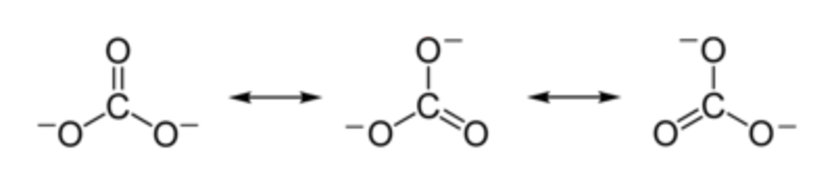
\includegraphics[width=0.6\textwidth]{Carbonate1.pdf} 
%\quad \quad \quad \quad  
%
\includegraphics[width=0.13\textwidth]{Carbonate3.pdf} 
%\end{center}
%\end{figure}
%
%Expérimentalement, on observe que l'ion se comporte comme un système symétrique en l'absence de champ extérieur. Pour rendre compte de ce fait expérimental, on imagine que la double liaison change de position en permanence : on modélise l'opérateur Hamiltonien de l'ion par
%\begin{equation}
%\hat H = E_0 \Big( \ketbra{\phi_1}{\phi_1} + \ketbra{\phi_2}{\phi_2} + \ketbra{\phi_3}{\phi_3} \Big) - \alpha \Big( \ketbra{\phi_1}{\phi_2} + \ketbra{\phi_2}{\phi_3} + \ketbra{\phi_1}{\phi_3} + h.c.\Big),
%\end{equation}
%où $E_0$ et $\alpha$ sont deux constantes réelles strictement positives. Supposons qu'au temps $t$, l'état du système soit $\ket{\psi(t)} = \frac{1}{\sqrt{2}}(\ket{\phi_1}+\ket{\phi_3})$. 
%\begin{enumerate}
%\item Déterminez une base d'états propres de l'observable $\hat H$. Cette base est-elle unique ?
%\item Calculez les résultats possibles auxquels peut conduire une mesure de l'énergie du système au temps $t$, ainsi que les probabilités associées. 
%\item Calculez l'énergie moyenne ainsi que l'incertitude sur la mesure de l'énergie au temps $t$. Montrez que l'une et l'autre sont constantes lorsque le temps s'écoule. Interprétez $E_0$ et $\alpha$.
%\end{enumerate}
%On souhaite à présent mesurer l'observable $\hat B$ définie par
%\begin{equation}
%\hat B = \beta \Big[3\ketbra{\phi_1}{\phi_1} + 2\ketbra{\phi_2}{\phi_2} + 2\ketbra{\phi_3}{\phi_3} +(1+\lambda) \ketbra{\phi_2}{\phi_3} + h.c.\Big],
%\end{equation}
%où $\beta$ et $\lambda$ sont des paramètres réels positifs.
%\begin{enumerate}
%\setcounter{enumi}{3}
%\item Analysez la structure propre de l'observable $\hat B$. À quelle condition $\hat B$ représente un invariant dynamique ? \textit{Indication :} calculez $[\hat B,\hat H]$.
%\item On mesure l'énergie du système et on obtient le résultat $E_0-2\alpha$. Quel est l'état du système après la mesure de $\hat H$ ? Évaluez alors $\Delta B$ dans cet état. Commentaires ?
%\item Supposons que nous disposions d'un appareil permettant de mesurer l'énergie et l'observable $\hat B$, dans cet ordre, et sans délai entre les mesures. Trouvez la probabilité d'obtenir le résultat $(E,B) = (E_0-2\alpha,3\beta)$.
%\item Imaginez maintenant que l'on mesure $\hat B$ avant $\hat H$, en retournant l'appareil. Quelles chances a-t-on de récolter le même résultat ? 
%\item Répétez les points 6 et 7 en supposant que $\lambda=0$. Qu'observez-vous ? 
%\end{enumerate}
%
%$ $

\paragraph{Exercice 7} \textit{Effondrement de la fonction d'onde.}\\
On considère le problème bien connu d'une particule libre de masse $m$ coincée entre deux plaques infranchissables situées en $x=0$ et $x=a$.
\begin{enumerate}
\item Soient $\ket{\phi_n}$ les états propres du système, associés aux énergies $E_n = n^2\pi^2\hbar^2/2ma^2$, $n\in\mathbb N_0$.
\begin{enumerate}
\item Calculez les éléments de matrice des opérateurs $\hat X$, $\hat P$ dans la base $\lbrace \ket{\phi_n}\rbrace$.
\item Déduisez-en les valeurs moyennes $\braket{\hat X}_n$ et $\braket{\hat P}_n$ ainsi que les incertitudes $\Delta X_n$ et $\Delta P_n$.
\item Vos résultats sont-ils compatibles avec la Relation de Heisenberg ? Évaluez l'énergie de point zéro du système, et comparez-la au résultat exact. 
\end{enumerate}

\item Initialement, l'état de la particule est $\ket{\psi(0)} = a_1\ket{\phi_1}+a_2\ket{\phi_2}+a_3\ket{\phi_3}+a_4\ket{\phi_4}$. On supposera, par un choix de phase adéquat, que $a_1$ est un nombre réel.
\begin{enumerate}
\item Quelle est la probabilité de trouver $E < \frac{3\pi^2\hbar^2}{ma^2}$ si l'on mesure l'énergie en $t=0$ ?
\item Calculez $\braket{\hat H}$ dans l'état initial, et déterminez l'incertitude sur la mesure de l'énergie. Quelles conditions sur les $(a_i)$ entraînent l'annulation de cette incertitude ?
\item Calculez l'état de la particule au temps $t>0$. Les résultats trouvés en (a) et (b) restent-ils corrects en un instant $t>0$ quelconque fixé ? Commentez votre réponse.
\item Lors d'une mesure d'énergie, on trouve $E=\frac{8\pi^2\hbar^2}{ma^2}$. Après la mesure, quel est l'état du système ? Quelle valeur obtiendra-t-on si l'on mesure à nouveau l'énergie ? Commentaires ?
\end{enumerate}
\item Considérons à présent que $a_1=a_2=\frac{1}{\sqrt{2}}$ et $a_3=a_4=0$. 
\begin{enumerate}
\item Écrivez la fonction d'onde $\psi(0,x)$ de la particule à l'instant initial $t=0$. Calculez la valeur moyenne de l'impulsion $\braket{\hat P}$, ainsi que l'incertitude sur la mesure de celle-ci.
\item Calculez l'état $\ket{\psi(t)}$ au temps $t>0$. Comment évolue la probabilité de présence $\rho(t,x)$ ? Montrez que la particule est conservée.
\item Montrez que le centre du paquet d'onde décrit par $\ket{\psi(t)}$ oscille autour de la position $x=a/2$ à une pulsation $\omega_0$ que vous calculerez. Commentaires ?
\item Calculez l'énergie moyenne $\braket{\hat H}$, ainsi que l'incertitude $\Delta E$ sur la mesure de l'énergie. Pour l'échelle de temps caractéristique du système $\Delta t = \omega_0^{-1}$, estimez $\Delta E\Delta t$.
\item Calculez la probabilité de trouver la particule entre $x=0$ et $x=a/2$ au temps $t$.
\item Supposons que l'on mesure l'énergie au temps $t_1$ et que l'on obtienne $E = \hbar^2\pi^2/2ma^2$. Quel est l'état du système en $t_2>t_1$ ? Supposons maintenant que l'on mesure la position du système en $t_2$, et que l'on obtienne $x=a/2$. Donnez la fonction d'onde \textit{normalisée} du système en tout temps ultérieur à $t_2$.
\item Quels résultats peuvent être retirés d'une mesure de l'énergie en $t_3>t_2$, et avec quelles probabilités ? Expliquez vos résultats.
\end{enumerate}
\end{enumerate}

$ $

\paragraph{Exercice 8} \textit{Ensembles complets d'opérateurs qui commutent.}\\
Soit $\hat A$ un opérateur hermitien agissant dans un espace de Hilbert $\mathcal{H}$. On peut prendre une base de $\mathcal{H}$ qui est constitué de vecteurs propres de $\hat A$. Si le spectre de $\hat A$ est non dégénéré, alors cette base est unique. Mais si le spectre est dégénéré, alors la base n'est évidemment pas unique ! Que faire ? Considérer une seconde observable $\hat B$ qui commute avec $\hat A$ ...
\begin{enumerate}
\item Montrez que $\hat A$ et $\hat B$ peuvent être simultanément diagonalisées si et seulement si $[\hat A,\hat B]=0$.
\item Montrez que, pour tout vecteur propre $\ket{a}$ de $\hat A$, $\hat B\ket{a}$ est également vecteur propre de $\hat A$.
Déterminez la valeur propre correspondante et expliquez les conséquences de ce résultat. 
\item Démontrez que $\bra{a_1}\hat B\ket{a_2}=0$ si $\ket{a_1}$ et $\ket{a_2}$ sont deux vecteurs propres de $\hat A$ associés à des valeurs propres \textit{distinctes}. 
\end{enumerate}

Grâce à ces résultats, on peut se munir d'une base dont tous les éléments sont à la fois vecteurs propres de $\hat A$ et de $\hat B$. Les différents vecteurs de la base seront désignés par la valeur propre de $\hat A$ et la valeur propre de $\hat B$. Si la base n'est toujours pas unique, on peut chercher un troisième opérateur $\hat C$ qui commute avec $\hat A$ et $\hat B$, et ainsi de suite, jusqu'à avoir, selon la formule consacrée, épuisé la dégénérescence. On définit alors un \textbf{E}nsemble \textbf{C}omplet d'\textbf{O}pérateurs qui \textbf{C}ommutent (\textit{E.C.O.C.}) comme une collection d'opérateurs hermitiens, tels que si l'on spécifie la valeur propre de chaque opérateur, on obtient un vecteur propre commun et unique. Cet exercice se fixe pour but d'étudier cette notion d'un peu plus près, au moyen de deux cas simples à traiter ! 

%\textit{Exemple} : pour l'atome d'Hydrogène, l'énergie des niveaux électroniques ne spécifient pas l'état de l'électron de manière unique. Par exemple, les orbitales $2s$ et $2p$ partagent la même énergie. Elles seront cependant différentiées par l'état du mouvement orbital de l'électron. Pour déterminer l'état de l'électron, il faudra ajouter à l'opérateur Hamiltonien des informations sur son état de mouvement autour du proton central, notamment la norme carrée de son moment cinétique orbital de l'électron, et la projection de ce dernier sur l’axe vertical. Il sera montré que ces trois opérateurs commutent et définissent une base d'états unique pour les orbitales électroniques. \\
%
%\\

\begin{enumerate}
\setcounter{enumi}{3}
\item On considère un système physique dont l'espace des états (à 3 dimensions) est rapporté à la base orthonormée formée par $\lbrace \ket{u_i} \rbrace_{i=1}^3$. Dans cette base, les opérateurs $\hat H$ et $\hat B$ sont représentés par les matrices
\begin{equation}
H =\hbar \omega_0 \,  \left[ 
\begin{array}{ccc}
1 & 0 & 0 \\ 
0 & -1 & 0 \\ 
0 & 0 & -1
\end{array} 
\right]
\quad ; \quad
B = b \, \left[
\begin{array}{ccc}
1 & 0 & 0 \\ 
0 & 0 & 1 \\ 
0 & 1 & 0
\end{array} 
\right], \quad \omega_0,b \in \mathbb{R}_0.
\end{equation}
	\begin{enumerate}
	\item $\hat H$ et $\hat B$ sont-ils hermitiens ?
	\item Montrez que $\hat H$ et $\hat B$ commutent. Donnez une base de vecteurs prores communs à $\hat H$ et $\hat B$. 
	\item Parmi les ensembles d'opérateurs $\lbrace \hat H \rbrace$, $\lbrace \hat B \rbrace$, $\lbrace \hat H,\hat B \rbrace$, $\lbrace \hat H^2,\hat B \rbrace$, lesquels forment un \textit{E.C.O.C.} ?
	\end{enumerate}

	\item On considère à nouveau un système physique dont l'espace des états (à 3 dimensions) est rapporté à la base orthonormée formée par $\lbrace \ket{u_i} \rbrace_{i=1}^3$. On définit $\hat L_z$ et $\hat S$ par leur action sur ces vecteurs de base :
	\begin{equation}
	\begin{split}
	&\hat L_z \ket{u_1} = \ket{u_1}, \quad \hat L_z \ket{u_2} = 0, \quad \hat L_z \ket{u_3} = -\ket{u_3}; \\
	&\hat S \ket{u_1} = \ket{u_3}, \quad \hat S \ket{u_2} = \ket{u_2}, \quad \hat S \ket{u_3} = \ket{u_1}.
	\end{split}
	\end{equation}
	\begin{enumerate}
	\item Écrivez les matrices représentant, dans la base $\lbrace \ket{u_i} \rbrace_{i=1}^3$, les opérateurs $\hat L_z$, $\hat L_z^2$, $\hat S$ et $\hat S^2$. Ces opérateurs peuvent-ils être considérés comme des observables physiques ?
	\item Donnez la forme de la matrice la plus générale représentant un opérateur qui commute avec $\hat L_z$. Même question pour $\hat L_z^2$, et $\hat S^2$. 
	\item $\hat L^2_z$ et $\hat S$ forment-ils un \textit{E.C.O.C.} ? Dans l'affirmative, donnez une base de vecteurs propres communs. 
	\end{enumerate}
	 
\end{enumerate}

\section*{Exercices complémentaires}
\vspace{10pt}

\paragraph{Exercice S1} \textit{Mesure et évolution.} \hfill
[\textit{Juin 2007.}] \\
Considérons un espace de Hilbert de dimension $2$ dont une base orthonormée est $\lbrace\ket{1},\ket{2}\rbrace$. Considérons l'état
\begin{equation}
\ket{\psi} = \frac{1}{\sqrt{3}}\left[ \ket{1} + \sqrt{2}\ket{2}\right].
\end{equation}
\begin{enumerate}
\item Supposons que l'on mesure $\ket{\psi}$ dans la base $\lbrace \ket{1},\ket{2}\rbrace$. Qu'entend-t-on par "mesurer dans la base $\lbrace \ket{1},\ket{2}\rbrace$" ? Quelles sont les probabilités de trouver les résultats 1 et 2 ?
\item Même question si l'on mesure $\ket{\psi}$ dans la base $\ket{\pm} = \frac{1}{\sqrt{2}} [\ket{1}\pm\ket{2}]$ ? Commentaires ?
\item Considérons l'opérateur hamiltonien $\hat H$ dont la représentation dans la base $\lbrace\ket{1},\ket{2}\rbrace$ est $H = 3\, E\, \ket{1}\bra{1} + E\, \ket{2}\bra{2}$. Interprétez physiquement la base $\lbrace\ket{1},\ket{2}\rbrace$. Si l'on prépare le système dans l'état $\ket{\psi}$ au temps initial $t = t_0$, écrire l'état du système au temps $t > t_0$.
\end{enumerate}
$ $

\paragraph{Exercice S2} \textit{Représentation P.} 
%Nous avons coutume d'exprimer les états d'un système en les projetant sur les espaces propres de l'opérateur position $\hat{\vec X}$, obtenant ainsi ce que les pionniers de la Mécanique Quantique ont baptisé \textit{fonction d'onde}. Cette représentation de l'état porte tout naturellement le nom de \textit{représentation X}. Nous utilisons aussi très souvent une représentation en termes des états stationnaires du système, laquelle est très utile pour étudier l'évolution des états quantiques. \\
%Cet exercice a pour but d'introduire une autre représentation très utilisée, qui consiste à utiliser les vecteurs propres de l'opérateur impulsion $\hat{\vec P}$ en lieu et place des vecteurs propres de position (\textit{représentation P}). Formellement parlant, les représentations $X$ et $P$ sont reliées par une transformée de Fourier entre les variables canoniquement conjuguée $(\vec x,\vec p)$. Nous verrons que cette représentation permet de trouver de manière élégante la solution de l'équation de Schrödinger pour une particule soumise à l'action d'une force constante.

\begin{enumerate}
\item On note $\ket{\vec p}$ le vecteur propre de $\hat{\vec P}$ de valeur propre $\vec p$. Déterminez les fonctions d'onde propres de l'opérateur $\hat{\vec P}$. Sont-elles normalisables ? Pourquoi ?
\item Calculez $\bar\psi(t,\vec p) = \braket{\vec p|\psi(t)}$ en fonction de $\psi(t,\vec x)$ définie à l'exercice précédent. Justifiez qu'en représentation $P$ le rôle de $\hat{\vec X}$ et $\hat{\vec P}$ sont échangés. Déduisez-en la forme de $\hat{\vec X}$.
\item Démontrez que $\bar\psi(t,\vec p)$ est normée si $\psi(t,\vec x)$ l'est (\textit{égalité de Parseval}).
\item Montrez que l'équation d'évolution de la fonction $\bar\psi(t,\vec p)$ en présence d'un potentiel indépendant du temps est
\begin{equation}
i\hbar \frac{\partial}{\partial t} \bar \psi(t,\vec p) = \frac{p^2}{2m}\bar \psi(t,\vec p) + \int \frac{d^3 q}{(2\pi\hbar)^{3/2}} \bar V(\vec p-\vec q)\bar\psi(\vec q,t) \label{eq:SchroRepP}
\end{equation} 
où $\bar V(\vec p)$ désigne la transformée de Fourier du potentiel $V(\vec x)$ et $p^2=\vec p\cdot\vec p$.
\item Considérons à présent un mouvement unidimensionnelle dans le potentiel $V(z) = -mgz$, où $m$ a les dimensions d'une masse, $z$ est l'altitude, et $g$ est l'accélération gravifique locale.
\begin{enumerate}
\item Exprimez le théorème d'Ehrenfest pour les valeurs moyennes de la position et de l'impulsion du mobile ponctuel. Comparez au mouvement classique.
\item Montrez que l'incertitude sur l'impulsion ne varie pas au cours du temps.
\item Écrivez la version uni-dimensionnelle de \eqref{eq:SchroRepP} pour ce potentiel linéaire. Déduisez-en une relation entre $\frac{\partial}{\partial t}|\bar\psi(t,p)|^2$ et $\frac{\partial}{\partial p}|\bar\psi(t,p)|^2$.
\item Intégrez l'équation obtenue et donnez à votre résultat une interprétation physique.
\end{enumerate} 
\end{enumerate}
$ $

\paragraph{Exercice S3} \textit{Petits problèmes à une dimension.} 
\begin{enumerate}
\item Considérons l'espace de Hilbert des fonctions $f : \mathbb R \to \mathbb C$ déclinantes à l'infini, muni du produit scalaire $\braket{f|g} = \int dx \, f(x)^*g(x)$.
\begin{enumerate}
\item Étudiez l'hermiticité des opérateurs $\hat X$ et $\hat D = \frac{d}{dx}$ et calculez $[\hat D,\hat X]$.
\item Montrez que l'opérateur $\hat A = i(\hat X^2+a^2\hat I)\hat D + i\hat X$ est hermitien pour tout $a\in\mathbb R$.
\item Trouvez l'état $\psi_0(x)$ du système tel que $\hat A \psi_0(x)=0$. Quelle est la valeur moyenne de l'impulsion dans cette configuration ?
\item Calculez la probabilité de trouver le mobile ponctuel décrit par $\psi_0(x)$ dans la région $-a\leq x \leq a$.
\item Un état excité du système est décrit par $\psi(x) = e^{i p_0 x/\hbar}\psi_0(x)$, où $p_0\in\mathbb R^+_0$. Calculez à nouveau la probabilité de trouver le mobile dans l'intervalle $-a\leq x\leq a$.
\item Donnez la valeur moyenne de l'impulsion de ce mobile dans l'état $\psi(x)$.
\end{enumerate}
\item Soient $\lbrace \psi_n(x) \rbrace$, les états stationnaires d'un système quantique correspondant aux niveaux d'énergie $E_n$ ($n\in\mathbb N_0$). Au temps $t=0$, une mesure de l'énergie donne $E_1$ avec une probabilité de $1/2$, $E_2$ avec une probabilité de $3/8$ et $E_3$ avec une probabilité de $1/8$.
\begin{enumerate}
\item Écrivez la formule la plus générale pour la fonction d'onde initiale $\psi(0,x)$.
\item Que devient cette fonction d'onde après un temps $t$, $\psi(t,x)$ ?
\item Montrez que la valeur moyenne de l'énergie dans cet état ne varie pas au cours du temps, et justifiez-le.
\item Calculez la densité de probabilité $\rho(t,x)$ ainsi que le courant de probabilité $J(t,x)$. Vérifiez que la particule est conservée.
\end{enumerate}
\item Soit une particule se déplaçant à une dimension aux dépens d'un potentiel $V(x)$ homogène de degré $n\in\mathbb N_0$ en $x$. 
\begin{enumerate}
\item Calculez la valeur moyenne du commutateur $[\hat H,\hat X\hat P]$ dans un état stationnaire.
\item Montrez que les valeurs moyennes $\braket{T}$ et $\braket{V}$ des énergies cinétique et potentielle, évaluées pour un état stationnaire également, satisfont l'égalité $2\braket{T}=n\braket{V}$ (\textit{Théorème du Viriel}). Vérifiez que ce résultat s'étend directement à 3 dimensions.
\end{enumerate}
\end{enumerate}

\paragraph{Questions d'examen:} 
\begin{itemize}[label=\textbullet]
	\item Systèmes discrets : Juin 2019 Q1, Août 2019 Q1, Juin 2022 Q3,
	\item Variables position et impulsion : Août 2021 Q2, Juin 2022 Q2.
\end{itemize}